\chapter{Result and Discussion}
In this chapter, we discuss about the results obtained from data analysis. First, we discuss about the cross section of ${}^{17}$B. In this analysis, we extracted the inclusive 2n removal cross section and 4n removal cross section. After that, we discuss about the relative energy spectra for ${}^{16}$B +n and ${}^{15}$B + n + n at Pb and C target. Also the angular distribution of scattering angle for ${}^{17}$B $\to$ ${}^{15}$B + n + n with Pb and C target is discussed. Finally, the result of Coulomb dissociation and B(E1) spectrum are discussed. Dineutron correlation is also discussed in this chapter.

\section{Cross Section}
\subsection{Inclusive Cross Section}
The inclusive cross section of ${}^{17}$B is obtained by following formula.
\begin{align}
    \sigma_{-xn} = \frac{\sigma_R - \sigma_R}{e^{-\sigma_R N_t} - e^{-\sigma_R N_t}} \bigg( \frac{N_{in}}{N_{in}} - \frac{N_{out}}{N_{out}}\bigg)
\end{align}


\begin{table}[h]
\centering
\begin{tabular}{c|c|c}
    \hline
     & $\sigma_{-2n}$ (mb) & $\sigma_{-4n}$ (mb) \\
    \hline
    $^{17}$B + Pb& 617(21) & 154(11) \\ 
    $^{17}$B + C & 159(3) & 63(2) \\ 
    \hline 
    $\sigma_{Pb}/\sigma_{C}$ & 3.9 & 2.4 \\ 
    \hline
\end{tabular}
\caption{Reaction Cross Section of Boron Isotopes}
\label{tab:Reaction Cross Section of Boron Isotopes}
\end{table}

\subsection{Coulomb Dissociation Cross Section}
Coulomb dissociation cross section can be extracted by using the following equation.
\begin{align}
\sigma_{CD} = \sigma_{inel}(Pb) - \Gamma \sigma_{inel}(C)
\end{align}
We used $\Gamma = 2.836$ from theoretical calculation. \cite{Ogata} 

\begin{table}[h]
    \centering
    \begin{tabular}[h]{c|c|c}
        \hline
         & $\sigma$  $E{rel} < 6$ MeV& $\sigma_{C}$ $E{rel} < 10$ MeV \\
        \hline
        Pb &  609(14)(60) mb & 450(10)(33) mb  \\
        C &  49(1)(8) mb & 32(1)(5) mb  \\
        CD &  470()(8) mb & 360()(8) mb \\
        \hline
    \end{tabular}
\caption{Coulomb Dissociation Cross Section}
\label{Coulomb Dissociation Cross Section}
\end{table}
In the Figure 5.1, the cross section for Pb and C target are shown. The blue dot is Pb target, and red dot is C target. The C target event is multiplied by $\Gamma$ Factor. In Figure 5.2, the coulomb dissociation cross section is shown. It has broad peak around 2 MeV.
\begin{figure}[h]
    \centering
    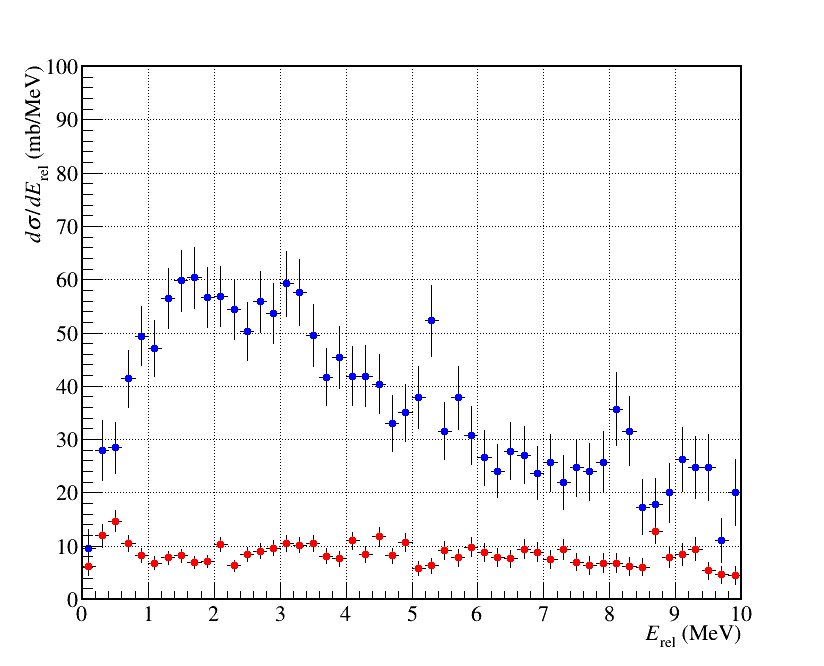
\includegraphics[width=11cm]{chapter5/coulomb_pb_c.png}    
    \captionof{figure}{Cross Section}
\end{figure}
\begin{figure}[h]
    \centering
    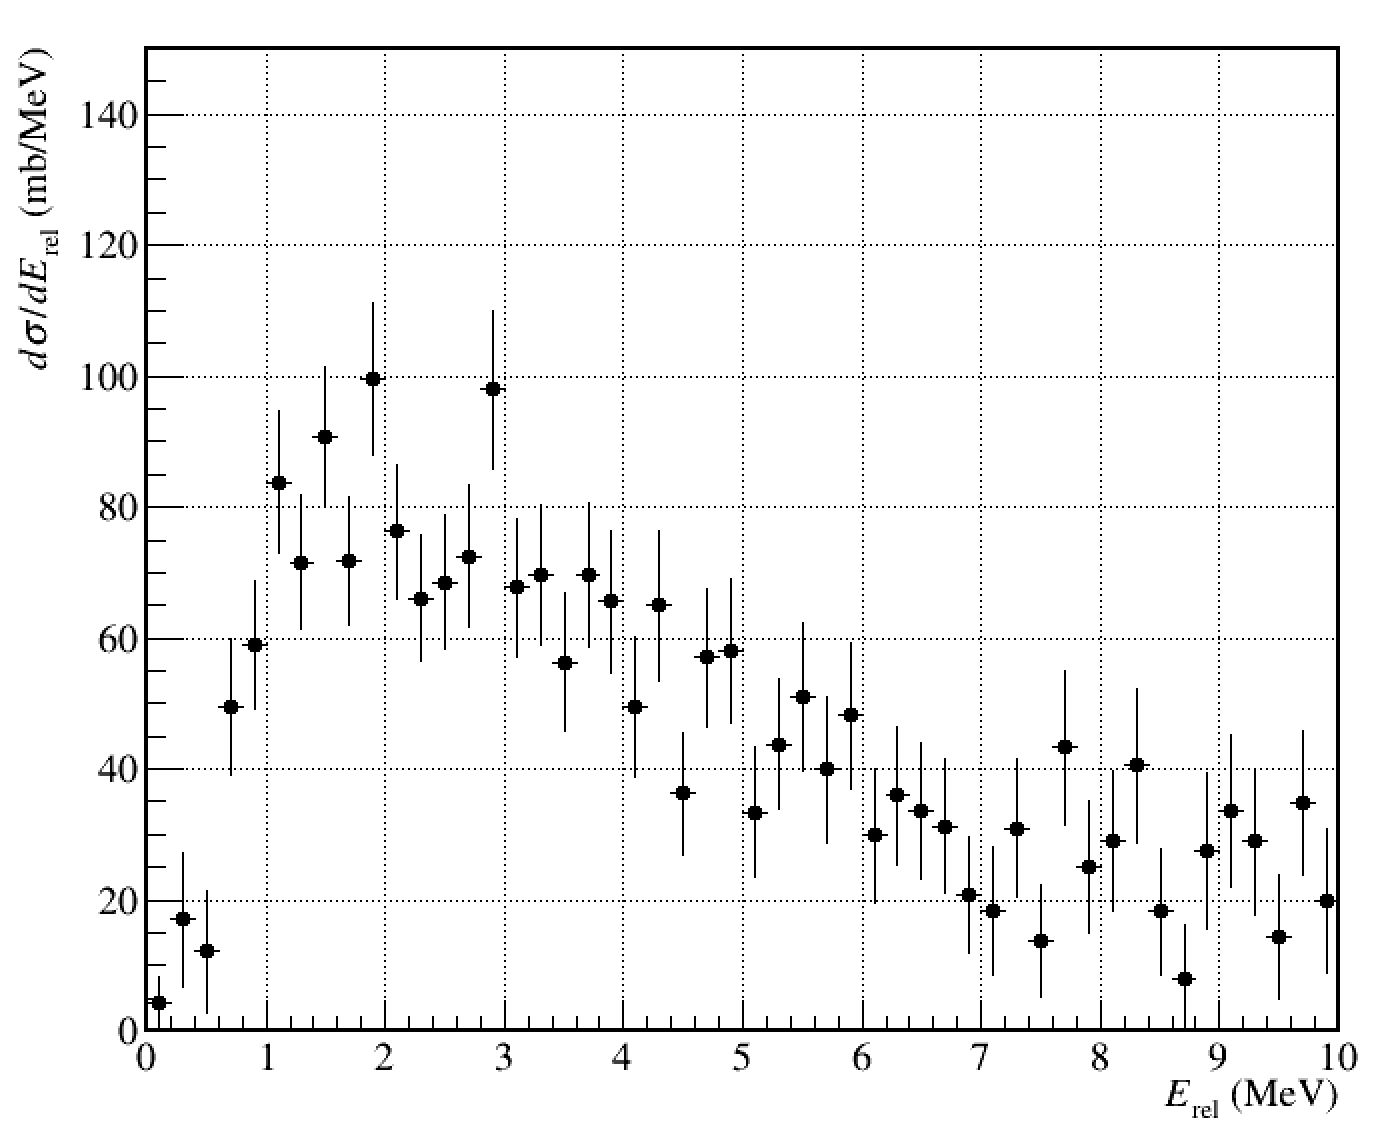
\includegraphics[width=13cm]{chapter5/dsigmadE.png}    
    \captionof{figure}{Coulomb Dissociation Cross Section}
\end{figure}    
\clearpage

\section{Reduced E1 Transition Probability}
About reduced dipole transition probability, we can extract $B(E1)$ strength as follows.
\begin{align}
    \frac{d \sigma_{coul}}{dE_x} = \frac{16 \pi^{3} }{9 \hbar c} N_{\text{E1}}(E_x) \frac{dB(\text{E1})}{dE_x}
\end{align}
The virtual photon number is calculated by using the formula (2.5).

\begin{figure}[h]
    \centering
    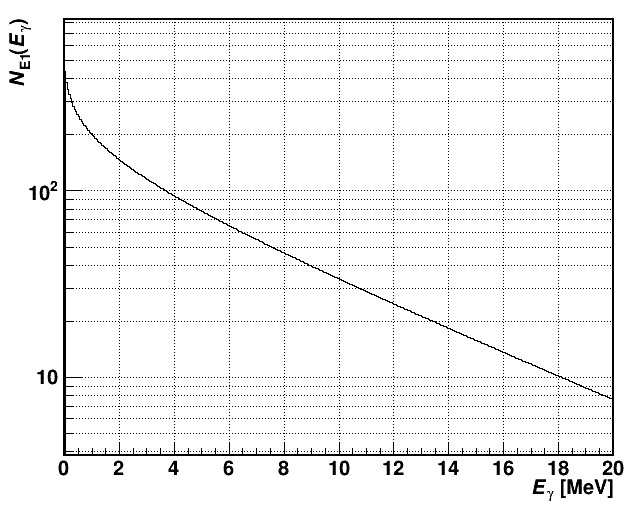
\includegraphics[width=10cm]{chapter5/virtual_photon_distribution.png}
    \captionof{figure}{Virtual Photon Number of ${}^{17}$B with 270 MeV/u at Pb Target}
\end{figure}
The reduced E1 transition probability B(E1) distribution is shown in Figure 5.3.
\begin{figure}[h]
    \centering
    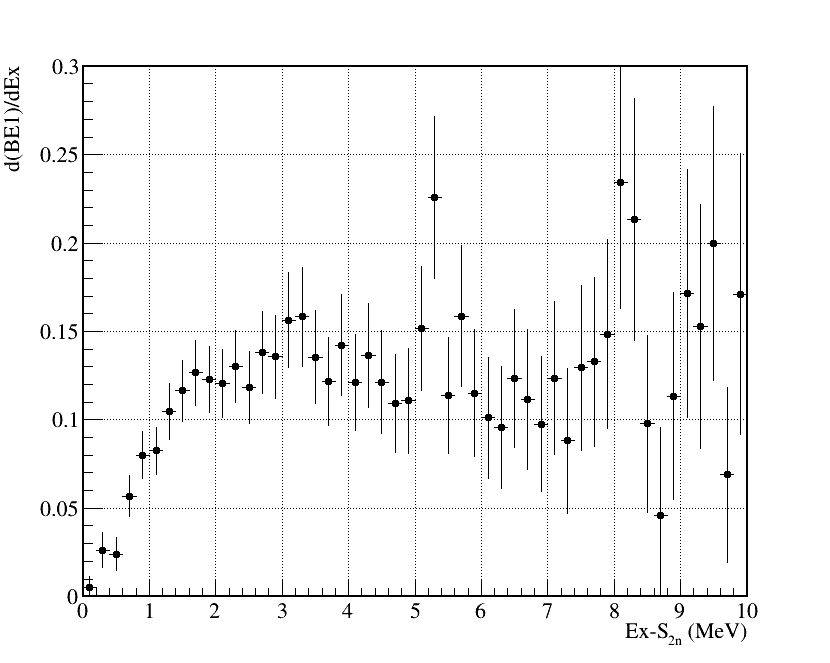
\includegraphics[width=13cm]{chapter5/dBdEx.png}    
    \captionof{figure}{B(E1) Strength}
\end{figure}  

\begin{align}
    B(E1) &= \int_{0}^{+\inf} \frac{dB(E1)}{dE_x} dE_x \\
          &\simeq \int_{0}^{+10} \frac{dB(E1)}{dE_x} dE_x = 2.04 \pm 0.10  [e^{2}fm^{2}] \\
          \\ \notag
          &\simeq \int_{0}^{+6} \frac{dB(E1)}{dE_x} dE_x = 1.16 \pm 0.05  [e^{2}fm^{2}] \\    
\end{align}  

\section{Dineutron Correlation}

\begin{align}
    B(E1) = \frac{3}{\pi} \bigg( \frac{Ze}{A} \bigg)^2 \langle r^{2}_{c-nn} \rangle
\end{align}
With the obtained $B(E1)$ strength up to 10 MeV, we can extract $\sqrt{ \langle r^{2}_{c-nn} \rangle}$ as follows.
\begin{align}
    \sqrt{ \langle r^{2}_{c-nn} \rangle} = 3.2 \pm 0.00 (stat.) \pm 0.00 (syst.) \text{ fm}
\end{align}
Furthermore, we can extract the distance of $2n$ from three body model.
\begin{align}
    \langle r^{2}_{halo} \rangle = \frac{A_c}{A} \langle r^{2}_{core} \rangle + \frac{2A_c}{A^2} \langle r^{2}_{c-nn} \rangle - \frac{1}{2A} \langle r^{2}_{nn} \rangle
\end{align}
where $A$ and $A_c$ is the mass number of halo nucleus and core. $\langle r^{2}_{h} \rangle$ and $\langle r^{2}_{c} \rangle$ are the mean-square matter radius of halo nuclei and the core, which is 3.00(6) fm and 2.75(6) fm respectively.
\begin{align}
    \sqrt{ \langle r^{2}_{nn} \rangle} = 6.57 \pm 0.00 (stat.) \pm 0.00 (syst.) \text{ fm}
\end{align}
Finally, the mean opening angle of dineutron can be extracted as follows.
\begin{align}
    \langle \theta_{nn} \rangle = 91.5 \pm 0.00 (stat.) \pm 0.00 (syst.) \text{ deg.}
\end{align}